\documentclass[tikz,border=8pt]{standalone}
\usepackage{tikz}
\usepackage{xcolor}
\definecolor{ink}{HTML}{16140F}
\definecolor{muted}{HTML}{6D675E}
\definecolor{honey}{HTML}{F0B429}
\definecolor{cream}{HTML}{E7E2DA}
\begin{document}
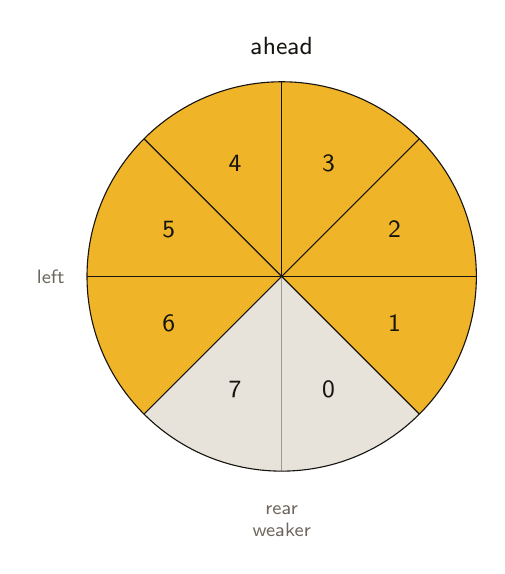
\begin{tikzpicture}[scale=1.15, font=\sffamily]
  \foreach \i in {0,...,7} {
    \pgfmathsetmacro{\a}{\i*45-90}
    \pgfmathsetmacro{\b}{\a+45}
    \pgfmathsetmacro{\mid}{\a+22.5}
    \ifnum\i=0
      \fill[cream] (\a:0) -- (\a:2.15) arc (\a:\b:2.15) -- cycle;
    \else\ifnum\i=7
      \fill[cream] (\a:0) -- (\a:2.15) arc (\a:\b:2.15) -- cycle;
    \else
      \fill[honey] (\a:0) -- (\a:2.15) arc (\a:\b:2.15) -- cycle;
    \fi\fi
    \draw[ink] (\a:0) -- (\a:2.15);
    \node[font=\sffamily\small, text=ink] at (\mid:1.35) {\i};
  }
  \draw[ink] (0,0) circle (2.15);
  \node[font=\sffamily\small, text=ink] at (90:2.55) {ahead};
  \node[font=\sffamily\scriptsize, text=muted] at (180:2.55) {left};
  \node[font=\sffamily\scriptsize, align=center, text=muted] at (-90:2.7) {rear\\weaker};
\end{tikzpicture}
\end{document}
